% !TeX root = ../all.tex


\section{Lower Bound on the Round Complexity}\label{sect:lb}


It seems obvious that using more batches will make it possible to use less samples, as the algorithm can more quickly adapt to its observations. What then is the precise relation between the sample complexity and the number of batches?

\citet{taoCollaborativeLearningLimited2019} focus on the problem of collaborative learning with limited interaction, in which multiple agents take samples in an environment and observe their own rewards, but must minimize the number of times they communicate their rewards with the other agents.
They manage to find a link, in some specific 2-armed instances, between how much faster an algorithm can get when communication is allowed, and the number of times the algorithm communicates.
They do so by constructing a sequence of gradually more difficult instances, each requiring one more batch than the previous one.
Generalizing this idea lets us reach the following result, for any pure-exploration problem.




\begin{restatable}[]{lemma}{theorec}\label{th:theorec}
	Suppose that a $\delta$-correct algorithm satisfies $\bP_{\bm\mu}\left(\tau_\delta >\gamma T^\star(\bm\mu)\ln(1/\delta)\right)\leq c$ for some $\gamma,c > 0$ on any Gaussian instance $\bm\mu$ with variance $\sigma^2$ with $T^\star(\bm\mu)\in (T_{\min},T_{\max})$.
	Let $(\bm\mu^n)_{0\leq n\leq N}$ be a sequence of such Gaussian instances with $T^\star(\bm\mu^n)=T^\star(\bm\mu^0)\zeta^{-n}\in (T_{\min},T_{\max})$ for some $\zeta\in (0,1)$.
	Then
	\begin{align*}
	&\bP_{{\bm\mu}^N}(R_\delta>N)
	\ge 1-N(2\delta+c)-\sqrt{\frac{\gamma\ln(1/\delta)}{2(\zeta^{-1}-1)}} S_n
	\end{align*}
	with
	\begin{align*}
	S_n = \sum_{i=0}^{N-1}\left[ 1+\sqrt{\frac{T^\star(\bm\mu^0)}{\zeta^{n}}\sup_{w\in \Sigma_K}\sum_{i\in[K]}w_i \frac{(\mu_i^{n+1}-\mu_i^n)^2}{2}}\right]
	\end{align*}
\end{restatable}

In order to get a lower bound on the number of batches, it remains to construct the right instance sequences for each problem.
It should start with an easy instance $\bm\mu^0$, and end with $\bm\mu^N=\bm\mu$ the instance whose complexity we want to study, with each succeeding instance being quantifiably harder than the previous one. See an illustration in Figure~\ref{fig:seqinst}.

\begin{figure}[!ht] \centering
	\scalebox{0.9}{
	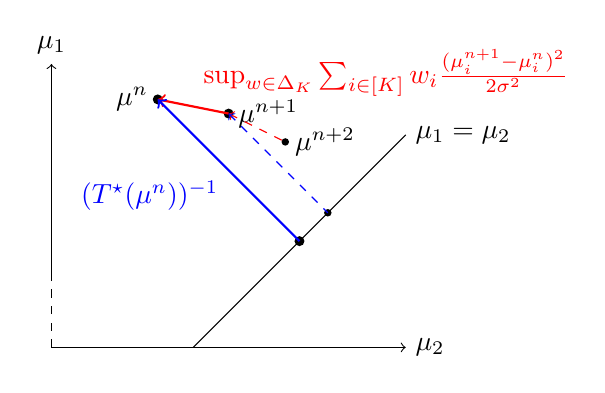
\begin{tikzpicture}[scale=0.9]
		
		% Draw axes
		\draw[->] (0,2) -- (5,2) node[right] {$\mu_2$}; % x-axis
		\draw[->] (0,3) -- (0,6) node[above] {$\mu_1$}; % y-axis
		\draw[dashed] (0,2) -- (0,3);
		% Draw the line y = x
		\draw (2,2) -- (5,5) node[right] {$\mu_1=\mu_2$};
		
		% Define points
		\coordinate (P1) at (1.5, 5.5);
		\coordinate (P2) at (2.5, 5.3);
		\coordinate (I') at (3.5,3.5);
		\coordinate (I2) at (3.3,4.9);
		\coordinate (I2') at (3.9,3.9);
		
		% Label points
		\fill (P1) circle (2pt) node[left] {${\bm\mu}^n$};
		\fill (P2) circle (2pt) node[right] {${\bm\mu}^{n+1}$};
		\fill (I') circle (2pt);
		\fill (I2) circle (1.5pt) node[right] {${\bm\mu}^{n+2}$};
		\fill (I2') circle (1.5pt);
		
		% Draw an arrow from (x,y) to (a,b)
		\draw[<-,thick,red] (P1) -- (P2) node[midway,above right] {$\sup_{w\in \Delta_K}\sum_{i\in[K]}w_i \frac{(\mu_i^{n+1}-\mu_i^n)^2}{2\sigma^2}$};
		\draw[<-,dashed,red] (P2) -- (I2);
		\draw[<-,thick,blue] (P1) -- (I') node[midway,below left] {$(T^\star(\bm\mu^n))^{-1}$};
		\draw[<-,dashed,blue] (P2) -- (I2');
		
	\end{tikzpicture}}
	\caption{Illustration of a sequence of instances}
	\label{fig:seqinst}
\end{figure}


An ideal sequence would minimize the sum $S_N$, thus allowing us to get to a larger $N$.
As getting such a minimizing sequence is difficult, we use simpler sequences $\bm\mu^n = \bm y +x^n(\bm\mu^0-\bm y)$ with $\bm y$ the constant vector $y_i=y\in \R$.
In order to be able to do so, an important ingredient is the following condition:

\begin{assumption}\label{asm:aff}
	For any mean vector $\bm\mu$, there exists $y\in \R$ such that for all $x \in (0, 1]$ and $\bm\mu' = x\bm\mu + (1-x)\bm y$ (where $\bm y$ is the constant vector $y$), $(T^\star(\bm\mu'))^{-1}=x^2(T^\star(\bm\mu))^{-1}$.
\end{assumption}

Top-k and thresholding bandits both satisfy that assumption.
With that condition, it is possible to simplify the bound of Lemma~\ref{th:theorec}. We give a general result for the exploration problems satisfying this condition in Appendix~\ref{app:lb}. We then apply this result to Top-k and TBP.	
	
\begin{restatable}[]{theorem}{thlbbaiexp}\label{th:lbbaiexp}
	For Top-$k$ and TBP, for a $\delta$-correct algorithm on Gaussian instances with variance $\sigma^2$ of complexity $T^\star\in(T_{\min},T_{\max})$, we have for any such Gaussian instance $\bm\mu$ of complexity $T^\star(\bm\mu)\in (T_{\min},T_{\max})$ that 
	\begin{align*}
	\bE_{\bm\mu}[R_\delta]
	&\ge \min\Bigg\{ \frac{\ln \frac{T^\star(\bm\mu)}{T_{\min}}}{2\ln\left( \left(\ln \frac{T^\star(\bm\mu)}{T_{\min}}\right)^2 \max\{e,C_\delta\}  \right)} \: ,\frac{1}{6}\ln \frac{T^\star(\bm\mu)}{T_{\min}},\frac{1}{6\delta}\Bigg\}
	\end{align*}
	with
	\begin{align*}
	&C_\delta = 1+4\gamma\ln\left(\frac{1}{\delta}\right)\ln \frac{T^\star(\bm\mu)}{T_{\min}}\left(1+\sqrt{\frac{T^\star(\bm\mu)\Delta^2}{\sigma^2}}\right)^2
	\: , \\
	&\gamma = \sup_{\bm\nu: T^\star(\bm\mu)\in (T_{\min},T_{\max})}\frac{\bE_{\bm\nu}[\tau_\delta]}{\ln(1/\delta)T^\star(\bm\mu)}
	\: .
	\end{align*}
	and where $\Delta = \frac{\max_i \mu_i -\min_i\mu_i}{2}$ in the Top-$k$ setting and $\Delta = \max_i |\mu_i - \tau|$ in thresholding bandits.
\end{restatable}

We give all details of the proofs in Appendix~\ref{app:lb}.
For $\delta$ small enough, the batch complexity is or order
\begin{align*}
\Omega \left\{\frac{\ln \frac{T^\star(\bm\mu)}{T_{\min}}}{\ln\left(\ln \frac{T^\star(\bm\mu)}{T_{\min}}\right) +\ln \left(\gamma \ln(\delta^{-1}) K\frac{\max_i \Delta_i^2}{\min_i \Delta_i^2}\right) }\right\}
\: .
\end{align*}
This is the first lower bound on batch complexity as a function of the sample complexity for all pure exploration problem satisfying Assumption~\ref{asm:aff}.
Our algorithm will have a batch complexity of order $\ln \frac{T^\star(\bm\mu)}{T_{\min}}$, almost matching the lower bound.

For collaborative bandits (where periods without communication are the analog of batches), \citet{taoCollaborativeLearningLimited2019} have worked on algorithms $\mathcal{A}_b$ satisfying $\bE_{\mathcal{A}_b}[\tau_\delta] =\cO\left( \inf_{\mathcal{A}}\bE_{\mathcal{A}}[\tau_\delta]\right)$, where the infimum is over fully sequential algorithms.
Their results can be adapted to the batched setting to show that there are two-armed instances on which those algorithms must satisfy $\bE[R_\delta]=\Omega\left( \frac{\ln\Delta_2^{-1}}{\ln(\ln\Delta_2^{-1})}\right)$.
Our result is valid for more pure exploration problems than just BAI; it is a bound on general $K$-armed Gaussian instances rather than specific two-armed instances; and gives instance-dependent bounds instead of merely the existence of an unspecified hard instance.

Theorem~\ref{th:lbbaiexp} does not contradict the guarantees of Tri-BBAI \citep{jinOptimalBatchedBest2023}. 
Their algorithm always uses 3 batches, but the sample complexity is only controlled in the regime $\delta\rightarrow 0$, in which our lower bound goes to $0$.
Since $\bE_{\bm\nu}[\tau_\delta]$ is not controlled otherwise, $\gamma$ can be large, making our lower bound small and consistent with $3$ batches.

\textbf{Necessity of $T_{\min}$}. The bound depends on $T_{\min}$, which is the minimal complexity for which the sample complexity of the algorithm is bounded by $\gamma T^\star(\bm\mu)\log(1/\delta)$.
Since no algorithm uses less than $1$ sample, every algorithm has such a $T_{\min}$ greater than $(\log(1/\delta))^{-1}$, and the lower bound is then of order $\log (T^\star(\bm\mu) \log(1/\delta))$.
$T_{\min}$ is a tradeoff between prior knowledge and batch complexity.
In the extreme situation in which $T^\star(\bm\mu)$ is known and the algorithm is $\delta$-correct only on instances of that complexity, the lower bound is 0.
Our algorithm will use at most 5 batches in that case: any lower bound has to be a small constant.
